
\chapter{Implementierung}
\label{chapter-implementierung}
Das folgende Kapitel beschreibt die Implementierung des Backends, Reservierungsinterfaces sowie des
Fontends. Zunächst wird ... beschreiben. Daraufhin wird ... beschreiben. Abschließend wird auf die
Inbetriebnahme des Systems eingegangen.


\section{Implementierung des Reservierungsinterfaces}
Der Abschnitt beschreibt die Struktur des Reservierungsinterface mit seinen technischen Aspekten
und die Implementierung der Funktionalitäten (\ref{section:funktionale}). Zunächst wird die
Implementierung der Kernfunktionalitäten erläutert. Daraufhin werden Sackgassen thematisiert.


\subsection{Struktur des Reservierungsinterface}
Das folgende Unterkapitel geht auf die Strukturen und Teilkomponenten des Reservierungsinterface
ein. In \ref{fig:db} wird die Verzeichnisstruktur präsentiert. Das Reservierungsinterface teilt sich
in drei wesentliche Bausteine: \textit{node, SQLit(prisma)} und \textit{server.ts} . 

\begin{figure}[h]
  \centering
  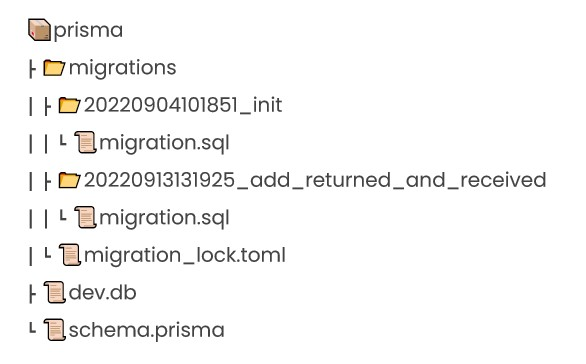
\includegraphics[scale=0.7]{Bilder/Db.jpg}
  \caption[Verzeichnisstruktur des Reservierungsinterfaces]{Verzeichnisstruktur des Reservierungsinterfaces}
  \label{fig:db}
\end{figure}

Der \textit{node} Ordner gibt... .

\textit{prisma} macht Dinge 

\textit{server.ts} für Routen

\subsection{Implementierung der Kernfunktionalität}
Dieser Abschnitt präsentiert die Implementierung der Kernfunktionalität des Zwischenbackends,
welche aus den Anforderungen  bestimmt wurden (\ref{section:anforderung}). Bei der Funktionalität
handelt es sich um das Reservieren in die Zukunft, sowie das Speichern dieser Vorgänge und die
damit einhergehende Bestätigung für die Aktualisierung in Snipe-IT.

Um auf die Assets zugreifen zu können wurde mit der Snipe-IT JSON REST API gearbeitet. 
Die api HIER AUFBAU ERKLÄREN.

Um mit der api arbeiten zu können muss ein \textit{API key} generiert werden. ERKLÄREN WIE MAN DEN
GENERIERT.

Durch die Nutzung von API key durch Snipe-IT lässt sich die  API nur per Token nutzbar, da die Token
nur manuell im Dashboard generierbar sind kann LDAP nicht ohne mega aufwand eingebunden werden.
Snipe-IT gibt zwar die möglichkeit, das LDAP Formular auszufüllen.. WEITER ERKLÄREN.


FÜR FRONTEND benötigte Ressourcen: Routen angelegt -> Fastify genutzt, für vereinfachung


Reservierung in der Zukunft: Daten zwischenspeichern, weil Snipe IT doof -> SQLite -> Prisma
  (für einfache verwaltung -> Beispeil und wie es Funktioniert) 


Statuseingabe/Ausleihen schwer und komisch -> rumarbeiten

\section{Implementierung des Frontends}
\begin{itemize}
  \item v-calender für den Kalender -> Kalender als wichtiger bestandteil -> viel ausbaumöglichkeiten
  \item Tailwindcss für das Styling
  \item Preline für UI -> Nicht empfehlenswert (Sackgassen)
  \item Headless ui für animation
  \item Basiskomponenten, für sich wiederholende und oft eingesetzte elemente
  \item Aufteilung mit dem Bindestrich: Kategorien im Frontend
\end{itemize}



Bei der Implementierung wurde sich an den best practices der
Vue.js-Dokumentation orientiert \todo{(Vue.js, 2021a)}. Zunächst wurde für die
in \ref{subsection:system} Components eine eigene View erstellt.


\section{Nutzung des Systems}
Um das System Nutzen und weiterentwicklen zu können muss...
API KEy generieren lassen

\section{Fazit der Implementierung}